\setchapterpreamble[u]{\margintoc}
\chapter{实验设计基本思想}
\labch{options}

\section{科学研究}
科学研究是是揭示物质世界的内在规律,寻求变量间因果关系。牛顿看到苹果自然而言地从树上掉下来,于是他思考,为什么苹果从树上向地上掉而不是向天上掉,当然苹果也可能就停留在空中.这就是物质世界的内在规律,这里例子中就是苹果落到地上和引起苹果掉落的原因。牛顿提出其原因是因为有重力,这个力的作用导致了苹果没有停在空中或者向空中掉的可能,这样把物质世界的规律找了出来,而且这个规律是通过引起与被引起这样的因果关系联系在一起的.同样地,心理学是研究人是如何认识并获取客观世界的知识的,并对人类的行为进行描述、理解、预测和控制.

鲁迅先生曾经写过:“一个人要想离开社会而生存,那正像拔着自己的头发想离开地球一样不可能”.心理学研究也是这样,我们用自己的大脑去研究存在于我们大脑中的心理,这种研究过程本身就是“纠着自己的头发离开地球”,看似我们完全不可能认识自己,但是在这么多年的沉淀中,已经积累了非常多的研究成果,这些进展都在告诉我们,人类的心理是可以研究的,我们是可以逐步深入地研究自己的心理的.下面以语言学习的例子,看看这种人类特有的符号系统人们是如何一步步进行研究的.

关于语言学习,其实每一个人都会有自己的体会,因为每个人都有语言。语言是人类最特殊的一种能力,要了解这种能力,只能通过人来做研究.虽然动物也有简单的交流,但是我们不可能通过动物来研究人的语言.科学家用什么样的方法手段,怎样去研究人类的语言呢?在过去的二三十年中,发生了巨大的变化。最初的时候,我们用行为的方法去研究,收集一些语言的现象,探讨语言的行为,通过反应时手段,推测大脑中语言加工的时间进程。近年来,研究者开始用一些非常精密、非常先进的仪器,包括眼动、计算机模拟、脑电、脑成像、基因的方法,这些方法让我们对人类语言的认识,特别是对语言学习发展、障碍及其脑机制的认识,有了非常重大的突破和进展。

儿童的语言学习是从什么时候开始发生发展的?如果有人接触过孩子的话,可以发现,孩子的语言发展是非常迅速的。从刚出生的时候一点都不会说,到一、
二、三岁以后,会说大量的词汇、语句。语言学家、心理学家已经对这个现象进行了大量的探讨,但到现在还是不能完全解释。学前儿童阶段通常是没有正规的语言教学的,但是语言的发展为什么这么迅速?动力在什么地方?机制是什么?这是语言学家、心理学家非常感兴趣的。另外,我们都知道,身高、体重是可以测量的,语言发展可以测量吗?有可能科学地测量哪个孩子语言发展得好,哪个孩子语言发展得差吗?我们是不是可以从儿童在学前时期的发展来预测孩子上学时候的阅读表现?特别是有语言和阅读困难的孩子,我们是否可能早期预测?这些都是特别吸引人的研究问题。

儿童语言是如何习得的是各国心理学家长期感兴趣的问题,其中一个重要的发现是,儿童在17~18个月左右有词汇爆发(vocabulary spurt, Bloom, 1985)的现象,即从17个月之前只能说出50个词以内,到20多个月能说出500或更多的词。词汇爆发的机制是什么?按照传统行为主义的观点,人毫无心理可言,所谓心理只是刺激与反应间的联结,所谓学习只是一个简单的刺激-反应见不断加固的过程,语言学习就成了在概念与词语间建立联结,并不断将这个联结强化的过程.但是按照这样的说法,词汇的增长速度应该是平稳增长的,不会出现这样的爆发现象.显然,人类的语言能力显然比行为主义认为的要复杂得多.

Noam Chomsky (1957)提出大脑里有专门的语言装置,叫LAD( Language Acquisition Device,语言获得装置/语言习得装置),人出生时就具有了掌握语言的天赋,外部语言环境会给语言装置设定参数,以便人类具体掌握一门语言.这个理论很好地解释了“词汇大爆炸现象”,当个体的LAD成熟时,就会开始接受外界的语言刺激并且极大丰富个体的语言能力.不过遗憾的是,将近一百年来的研究并没有找到LAD在哪里.我不禁想问:这种假设还有可能被证明吗?以前我们认为几乎是不可能的。现在,脑科学发展以后,这个答案被揭开开始变得可行了,我们越来越接近了解更多的东西。比如下面这个实验,揭示了新生儿一出声时他的语言及其脑基础是什么样的,是一片空白?还是说人类先天就能把语言与别的声音区分开来?

Daniela Perani等(2011)给出生刚刚两天的新鲜婴儿做FMRI,让他们在睡觉的时候听故事,听的是女声讲的母语故事。这个实验设计有三个条件,第一个条件是给新生儿听的是正常的母语故事;第二个条件是新生儿听到的是只有声调,即将正常的声音去除了声母、韵母,只剩下声调;第三个条件是把声调拉平,音节、声母、韵母仍然保持。科学家希望了解当新生儿听这三种不同的声音时,他们的大脑会有反应吗?在哪里反应?

结果在\reffig{Perani(2011)1}中可以清楚地看到,如果在只有声调的条件下,新生儿大脑两侧都不反应;如果是拉平声调的条件,没有声母、韵母,大脑也不反应;只有在听正常故事的时候,新生儿大脑才有反应。新生儿是真的能听故事吗?研究表明,新生儿不是真的能听故事,他的大脑主要是对人的正常语音进行反应,对语义是不反应的。

\begin{figure*}
	\includegraphics{Perani(2011)1}
	\caption[Perani(2011)1]{Perani(2011)给两天大的婴儿听三类声音,记录他们的脑部激活情况,结果显示婴儿天生对语言有特异性加工,对非言语声音不产生反应.}
	\labfig{Perani(2011)1}
\end{figure*}

进一步的研究结果如\reffig{Perani(2011)2},还发现新生儿大脑的主要反应区是在大脑双侧的颞叶,是对语音、基本声音反应的脑区,而语义加工的脑区是不激活的。与成年人的语言加工主要在左半球相比,新生儿的语言加工是双侧的。因此我们至少能知道,新生儿出生的时候,大脑皮层已经开始对语音产生反应了.

\begin{marginfigure}
	\includegraphics{Perani(2011)2}
	\caption[Perani(2011)2]{Perani(2011)发现新生儿的语言加工主要是双侧,而成年人的语言加工主要是左半球}
	\labfig{Perani(2011)2}
\end{marginfigure}

更进一步的研究中,Perani对比了新生儿和成年人听觉中枢的发展情况,如\reffig{Perani(2011)3}中看到的那样,成年人的颞叶和额叶(A中绿色和黄色区域)见有丰富的白质纤维束连接(蓝色区域),而新生儿额叶和颞叶间的联结确不那么紧密, 这表明婴儿只对语音起反应,几乎没有对更高级的语义和语法加工,而建立起这个联系的主要途径就是接受丰富的语言刺激.

\begin{figure}
	\includegraphics[width=1\textwidth]{Perani(2011)3}
	\caption[Perani(2011)3]{Perani(2011)对比了婴儿和成人听觉中枢的情况,发现婴儿颞叶到额叶见的联系只是初步建立,还不完善,由此推断新生儿只是听声音,但并不明白其含义.}
	\labfig{Perani(2011)3}
\end{figure}

上面这个系列实验是在实验室中通过严格的控制得出的结论,事实上,并不是只有在实验室中的实验才是科学实验,重要的是科学研究的思想。我们先简要说说\textbf{科学研究的思想},随后看看非实验室的研究可以怎样的出科学的结论.

\begin{description}
    \item[1.系统的理论框架]
    只有有了系统的理论支持,收集数据才不是盲目的,上述实验中如果不是有Chomsky的理论支持,我们不会新生儿的语言获得情况有所兴趣,如果不是因为有FMRI研究技术的发展,我们不会想到用多功能核磁对新生儿进行研究.毕竟,一个刚出生两天的小婴儿,要其主观报告或者用其行为指标来反应其是否对语言有反应是不可能的.研究不是没有目的收集数据,而是有一定的理论支持,有一定的研究目的;
    \item[2.控制机制]
    主要是说的对无关变量进行控制,这一点和第三条一起说比较方便;
    \item[3.对象之间的因果关系]
    因果关系是心理学研究中最想得到的,想要做到为点需要有严格的控制.最理想的情况是研究者操控自变量在不同水平,并且控制无关变量,再对因变量进行观测,这样获得因变量观测值的差异就是由研究者在实验中让被试产生的,就可以很肯定的说是由自变量的变化导致的.关于这点我们还要再以后自变量的分类上谈,但此处要留个印象:最严格的因果关系是建立在实验中研究者人为造成的使被试形成的差异,比如上实验中输入的语料类型让婴儿由研究者的操作而导致的它们语言加工产生差异,这种差异是在实验室内产生的,是研究者明明白白控制了的,动因明确的.有些被试间的差异不是由研究者引起的,造成这个差异的原因也千奇百怪不得已而知,因此这类自变量往往不能得出严格的因果关系,比如说性别.因为行为学实验个体差异的关系,因此研究者通常用被试内设计,也就是一个被试要接受所有的处理,这样可以有效分离出被试间个体差异,这点我们后面要细谈,此处提及只是因为上实验(Peranti,2011)用的就是被试内实验设计,每个婴儿都听了这三段音频.
\end{description}


接下来我们以“对儿童说谎行为的研究”谈谈\textbf{科学研究目标}:

\begin{description}
    \item[1.描述]:如观察儿童说谎行为的各种不同表现形式、说谎的频率;
    \item[2.理解]:了解儿童说谎的原因(是否为了逃避批评或惩罚、或者为了获得某种利益?).我们知道儿童想要说谎必须有一定的认知机制,说谎不是一个简单的事情, 要有一定的认知能力才能说谎.要知道别人对问题是怎么想的,考虑别人怎么看问题才能说出来看起来比较严密的谎言,认知能力还没成熟的孩子说的谎在成年人看起来往往是可笑的;
    \item[3.预测]:什么样的家庭或学校环境下,什么年龄儿童可能出现说谎行为;
    \item[4.控制]:如果已经知道孩子在青春期喜欢说谎,并且这个现象不利于孩子的发展,那是否可以有合理的控制机制让说谎情况降到最低呢?
\end{description}


下一步,我们继续讨论\textbf{心理学研究的途径},此处不会详细论述某种研究手段,想向各位传达的信息是,不是只有典型的实验研究才是研究,别的研究手段尽管没有对实验条件进行严格的控制,但这些手段都是科学的,都是为了一定的研究目的服务,也会进一步深入问题提供一个基础.额外想提醒的是,研究手段和研究目的紧密相关,有些现象没法用实验的手段,这点我们也放到后面的实验设计中谈.

\textbf{1.观察}

观察法指的是在自然状况下收集数据,描述某种现象包括自然现象,包括自然观察,问卷调查,个案研究.前面我们提到了儿童一岁半左右一个很有趣的词汇暴增现象——\textbf{词汇爆炸(vocabulary spurt)}.Bloom(1985)首先在国外儿童中发现了这个现象,那么中国儿童是否也存在这个现象呢?这就有赖于对汉语母语儿童的观察,我国学者确实发现在汉语母语儿童身上也发现了相同的现象(Li, 2007),下面介绍一下他们的研究.我们没法对6-7个月的儿童进行控制,让他们主观报告自己会说的词汇,因此只能让家长填写词汇问卷,判断哪些词是自己孩子说过的.这个词表数目还挺多的,让一个家长做完整个词表会造成较大的疲劳效应,因此实验中也匹配了一些“平行家长”,不过这都是控制机制,在此我不打算具体介绍.总之,在\reffig{Li(2007)}中我们确实看到,在18个月左右时,确实存在一个词汇量剧增的时间点.

这个实验中,我们不是被动的收集数据,而是有着某种特殊目的收集儿童的词汇量,并且这个实验结果得到了一个漂亮的结果.可见,描述性实验也失为一种有用的科学实验

\begin{figure}
    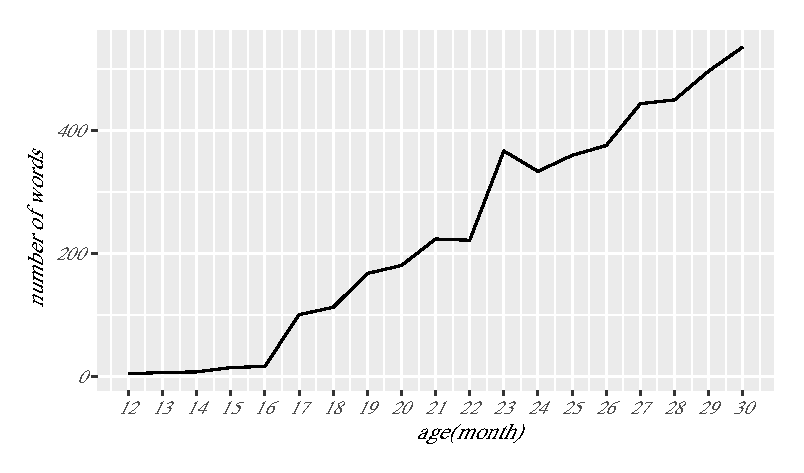
\includegraphics[width=0.8\textwidth]{Li(2007)}
    \caption{Li(2007)对12到30个月的汉语母语儿童进行了词汇量的追踪,结果发现了他们身上也存在词汇爆炸(vocabulary spurt)现象}
    \labfig{Li(2007)}
\end{figure}

\textbf{2.相关研究}
相关研究对两种现象(变量)之间的关系感兴趣,例如:吸烟与肺癌之间的关系.但是没法指因两个变量间引起与被引起的方向(到底吸烟引起肺癌,还是有肺癌基因的人倾向于吸烟不能从显著的相关中推论)

在对儿童语言发展的研究中,我们感兴趣的是孩子抚养人(特别是母亲)的语言使用清空对孩子会有什么样的影响,具体来说,父母寡言是否孩子也会寡言?父母受教育程度高是否导致孩子更喜欢说话?处于伦理道德的限制,我们只能记录孩子和父母的情况,不能对上述两个因素进行严格控制.

这个问题一直不能好好解决,因为要对一段录音中词语数进行统计是相当困难、工作量巨大的事情.不过LENA技术的出现让这种困境得以摆脱.这个程序可以识别婴儿的声音中的语言成分,并把一些非言语部分分离出去,比如哭声、吃东西的声音;它还可以分辨不同人的声音,这样也可以家长的说话情况.

这个实验的结果如\reffig{LENA}所示,我们能非常清楚地看到,父母地寡言和多言确实影响了孩子的与发展,
 
\begin{figure*}
    \includegraphics{LENA}
    \caption{用LENA研究父母多言寡言与受教育程度与孩子语言发展情况,结果发现这二者都和孩子的词汇发展成正相关}
    \labfig{LENA}
\end{figure*} 
 
\textbf{3.实验研究}

以Hagoort(2004)的一个研究为例看看他精细的设计.我们已经知道语义违反\sidenote{语义违反(semantic violation),指的是合乎语法要求却不符合词语的意义,如“这本书很咸”,从句法来看这句话是正确的,但是“咸”这个形容词不能修饰不是食物的名词,因此此处属于语义违反句子}会引起N400.还有一类句子错误,虽然语法、语义上都是正确的,但是和我们关于这个世界的认识是相违背的,比如“中国国家主席是位女士”.上述的两类错误涉及两种句子理解过程,一个是语义理解,一个是世界知识理解,以往人们认为这是两个独立的过程.Hagoort指出实际上这两种过程的区别不太好分开,因为很多词语都是不止有一个意思,多义词在特定语境中是什么意思要用世界知识来判断,进而Hagoort判断,世界知识违反(world knowledge violation)也会引起N400.

\begin{marginfigure}
    \includegraphics{dutch_train}
    \caption{荷兰火车的配色,实际上的车型并非如此}
    \labfig{dutch_train}
\end{marginfigure}

实验的材料(见\reffig{Hagoort(2004)}中的文字)经过了精心的设计,Hagoort给世界知识违反、语义违反、正确句子下了三个操作定义,这里用了一个非常有意思的操作定义来表示世界知识违反:实验的被试都是荷兰人,荷兰的火车都是黄色为主色调的(配色类似\reffig{dutch_train}),因此“The dutch trans are white”显然不符合荷兰人心中存在的对火车的知识.结果非常证实了Hagoort的猜想,在\reffig{Hagoort(2004)}可以清楚地看到,正确句子没有引起N400,而语义违反和世界知识违反都引起了N400.

\begin{kaobox}[frametitle=问题:如果这个实验只保留世界知识违反和正常条件,可行吗?]
如果顺着这个实验的结果来推理,这么做是看起来是可行的:把这个实验结果上的语义违反条件去掉,世界知识违反也确实引起了N400.但是要注意,实验前研究者并不知道结果是什么.也就是说实验前的假设是:\\
(1)若世界知识违反可以引发N400,说明语义理解与世界知识理解是一个连续的过程;\\
(2)若世界知识违反没有引发N400,说明语义理解与世界知识违反是两个独立的过程.\\
如果没有语义违反条件,(1)的结论还是可以得出,但是(2)中似乎存在了点问题.因为实验结果不显著不一定是处理效应不存在,还可能是检验力低的问题.对于心理学实验,它的处理效应本身就不高,那些不太明显但是确确实实存在的现象才有研究和发掘的价值.因此处理效应的显著需要较高检验力,实验设计一定要尽力精准和敏感.但不是所有实验都可以做到那么精准,想要得到漂亮的结果不是一件容易的事.在本实验中,如果没有语义违反做对照,在世界知识违反不显著时,研究者没法区分这是由实验不敏感导至的,还是由处理效应不存在导致的.因为语义违反已经被无数实验证明一定会引起N400,所以加上语义违反这个条件,就可以对实验的敏感性进行检验.这样(2)就可以拆分为以下两个假设:\\
(1)若世界知识违反没有引起N400,语义违反没有引起N400,则说明实验不够敏感,需要重新设计实验,处理效应是否存在有待继续检验;\\
(2)若世界知识违反没有引起N400,语义违反引起N400,则说明世界知识范围确实不会引起N400,世界知识违反和语义违反是两个独立的过程.
\end{kaobox}

\begin{figure}
    \includegraphics[width=1\textwidth]{Hagoort(2004)}
    \caption[Hagoort(2004)]{Hagoort(2004)给被试看三个句子并记录其脑电,发现世界知识违反的句子也会引起N400,进而说明了语义理解与世界知识理解是一个整体而不可以分割的过程.}
    \labfig{Hagoort(2004)}
\end{figure}

分析一下这个实验为什么是一个好实验.首先在自变量研究者控制了关键词的不同,在无关变量的控制上,除了关键词以外的句子都一摸一样,这样就排除了由于文字本身难度、熟悉度、使用频率带来的无关变异.实验设计上,采用被试内实验设计,每个被试都读了这三个句子,控制了所有的被试间的差异.这样总得来看,操作定义下得很精准、无关变量控制得也很巧妙,是一个值得我们学习的非常典型的实验设计.

\section{心理学实验设计基本问题}

从上面的实验可以看到,\textbf{心理学实验的特点}是:

(1)影响因素多;(2)因素之间相互关联;(3)无关变量的混淆

研究者在操纵和改变自变量时候,有大量无关变量,有这么多复杂的因素需要控制,行为实验中最复杂的因素,这也是以人研究对象的实验的难点.当然我们也非常自豪地说,这是心理学家最擅长的.

我们接下来讨论什么是\textbf{实验设计}.广义的实验设计涉及的内容比较广泛,此处不予以介绍,我们看看狭义的、典型意义的实验设计要做什么.狭义的实验设计就是做好实验的计划方案、统计分析方案,就像盖房子需要一个蓝图,我们不能在盖房子前什么规划都不做就直接去盖,同样我们也不能没有计划就去进行一个实验.实验之前要做一个详细的规划,这非常重要.如果这个方案没有做好,之后便很难纠正.

\textbf{实验设计的主要目标}有三点,首先,要回答感兴趣的理论问题;其次,要获得更加丰富的信息;最后,要提高的敏感性.我们分别来看看这些目标的具体含义:

\begin{description}
	\item[1.回答感兴趣的理论问题] 
	~\
	前面已经提到了,我们感兴趣的问题是人类心理现象的规律性问题,也是对人类行为和心理现象产生的动因感兴趣.所以首先我们要建立变量之间的关系,在实验中操纵或改变一个或多个变量,并观察其对行为的影响,记录下因变量的观测指标的变化情况.
	
	但是影响某个心理或行为的因素不只有我们感兴趣的自变量那么简单,我们的想法是让不同被试仅仅在自变量上有所不同,并且这个不同是由研究者操纵的,这样结果就确定是由自变量引起的.但由于实验对象的特殊性,我们很难保重不同人在进行实验前是完全相等的,所以我们还要对那些对因变量也产生影响,但是不是为研究者所感兴趣的变量进行控制,也就是要控制无关变量,减小或控制其对因变量影响.
	
	最后,选用复杂的统计方法,在同样的数据量中得到更多有意义的信息.
	
	\item[2.更加丰富的信息]
	~\
	首先,可以选用更好的实验设计的种类,比如在多因素设计中,除了主效应,还有交互作用,而交互作用往往可以提供一些非常有用的信息.在研究中,不同因素间往往存在相互影响,忽略一个因素而研究另一个因素时,难以看到真实的结果,这就是单因素实验设计的局限.
	
	其次,可以选用丰富的因变量,这个等下举个例子说明.
	
	最后,正确选择一些复杂的统计
	
	\begin{kaobox}[frametitle=多因素实验设计的优点]
		~\
		(1)可以同时估计两个或多个实验处理的效应,可以估价实验处理之间的交互作用
		
		(2)因素实验设计可以对数据资源进行更加有效的利用,使同样数量的数据给出丰富的信息
		
		但是要注意的是,多因素实验设计的统计和解释可能会比较复杂,特别是对于一个高次的交互作用,很难解释其意义;并且,过多因素的实验设计可能设计时觉得还挺漂亮的,但是实际做出来交互作用都不显著.这提醒我们研究一个问题的时候要先深入研究该领域,,当有足够了理论支持多因素实验的交互作用显著时,多因素实验设计才可能成功.
	\end{kaobox}

	\item[3.提高实验的敏感性] 
		~\
		前面我们已经提到,处理不显著的时候,可能真的是处理效应不存在,也可能是实验设计不够敏感,我们要尽量减小后一种的可能性.不过大多时候如果处理效应不显著,我们并不能将这两者区分开来.
	
\end{description}



%记得整理一下这个实验=-= 还要自己画图嘤嘤嘤

%舒华(1996)的五张图
%字的类型和年级交互作用
\begin{marginfigure}
	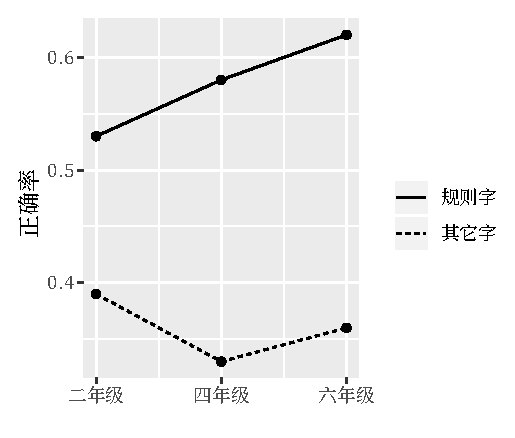
\includegraphics{shu(1996)_grade_type}
	\caption{字的类型$\times$年级}
	\labfig{shu(1996)t_g}
\end{marginfigure}

%字的类型和熟悉性交互作用
\begin{marginfigure}
	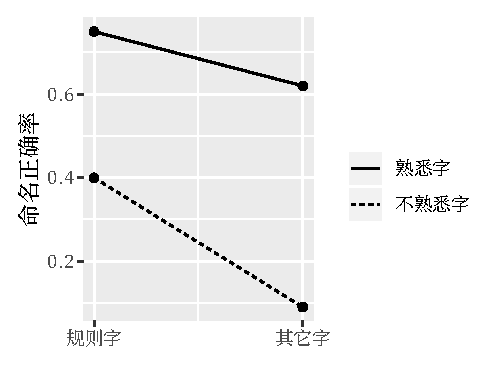
\includegraphics{shu(1996)_type_familiarity}
	\caption{字的类型$\times$熟悉性}
	\labfig{shu(1996)t_f}
\end{marginfigure}

%能力/熟悉性/类型三次交互作用图(重要! 好好解释)
\begin{marginfigure}
	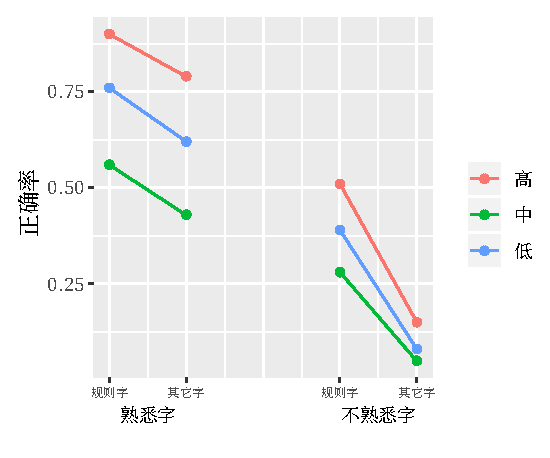
\includegraphics{shu(1996)_familiarity_type_capicity}
	\caption{能力$\times$熟悉性$\times$字的类型}
	\labfig{shu(1996)_t_f}
\end{marginfigure}

%错误分析
\begin{marginfigure}
	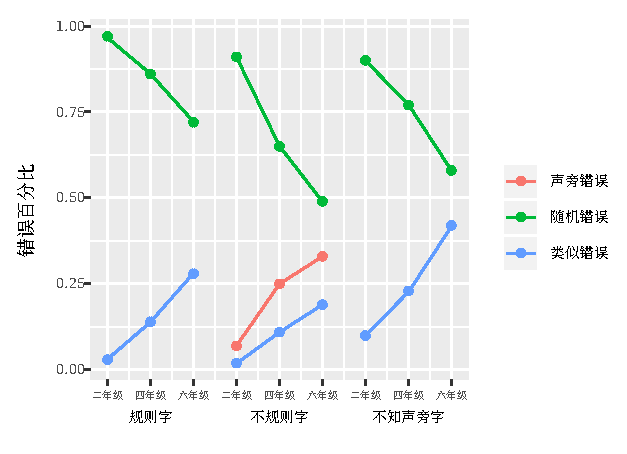
\includegraphics{shu(1996)false}
	\caption{儿童在各类字读音中犯不同类型错误占总错误的百分比}
	\labfig{shu(1996)_false}
\end{marginfigure}


%读音错误分析
\begin{marginfigure}
	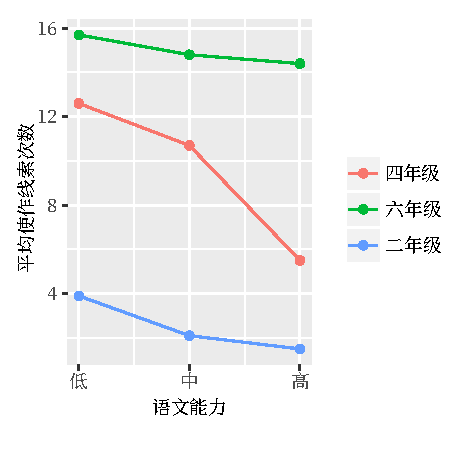
\includegraphics{shu(1996)_grade_capicity}
	\caption{儿童读音中使作线索的平均次数}
	\labfig{shu(1996)_cue}
\end{marginfigure}

舒华(1996)的一项研究中,对孩子读汉字的过程进行研究,特别是不熟悉的汉字.研究者想看到孩子读汉字能力的发展.实验中有一个非常漂亮的三次交互作用,揭示了一下有价值的信息.

这是一个3(年级)$\times$3(语文能力)$\times$2(字的熟悉性)$\times$3(字的类型)的四因素混合设计,其中字的熟悉性和字的类型是被试内变量,语文能力和年级是被试间变量.实验材料是60个单个形声字组成的卷子,所有的字都选自小学语文课本,每个年级的卷中包括30个熟悉的字和30个不有不同的字.熟悉字指学生在课本中已经学过的字,不熟悉字指学生在课本中还未学过的字,例如四年级卷子中的熟悉字选自第五、六册语文课本(三年级用书)后面的生字表,不熟悉字选自第九、十册语文课本(五年级用书)后面的生字表.每种熟悉度的字中有10个规则字,即字的声旁本身是一个儿童熟悉的汉字,且声旁的读音与字的读音相同,如“绘”;10个不规则字,即字的声旁是一个儿童熟悉的汉字,但声旁的读音与字的读音不相同,如“略”;和10个不知声旁的字,即字的声旁不是一个独立的汉字,其读音是一般人所不熟悉的,如“忱”,它的声旁“冘”的读音是“yin2”.不同熟悉度和不同类型的字的笔划数是经过匹配的,平均笔划数为10.实验是在三个自然班中集体进行的,每个学生接受相应年级的卷子,并按要求用拼音给出30个熟悉字和30个不熟悉字的读音,对写不出准确拼音的字,可以写一个与它同音的熟字代替. 

上述几个自变量比较难操作的是熟悉性.熟悉是最熟悉、全部都认识的吗?不熟悉、一定不认识的吗?这样做的话会出现天花板和地板效应,也就是熟悉的字成绩为100\%,不熟悉的字成绩为0.比较好的实验设计是,熟悉是比较熟悉,但也不是百分之百熟悉;不熟悉是相对不熟悉,也不是0.额外,上面提到,不同年级的材料间有一定的重叠这样使用的汉字数量比较少,这就减少了由汉字本身特点带来的无关变异.最后二四六年级的儿童匹配到的熟悉和不熟悉汉字的来源是:

\begin{figure}[hb]
	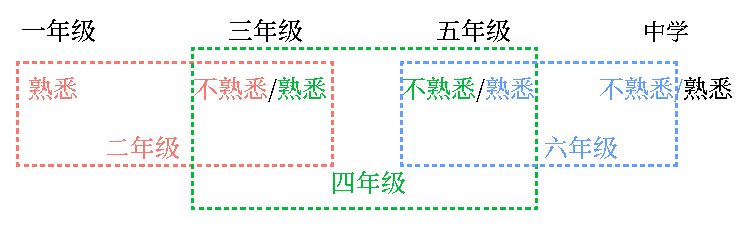
\includegraphics{shu(1996)_meterial}
	%\caption{舒华(1996)对二四六年级儿童熟悉字和不熟悉字的定义}
	\labfig{shu(1996)_meterial}
\end{figure}

年级和字的类型的交互作用显著(见\reffig{},规则字随着年龄增长,不规则字差不多,使用这个规则有一个学习过程

字的类型和熟悉性的交互作用显著,不规则的字更倾向于推理

语文能力三次交互作用显著,不熟悉的字中

对错误的分析中,三类
随机错误三类错误都下降
不规则字声旁错误增加
类似错误也是增加的
儿童对汉字的认知在发展,光读声旁很可能读错,所以在家族中找一个字

使用线索的次数,四年级有一个较大的发展

正确率由前侧,50\%正确率有较大变异

%-----------------------------------------------------------------
想要达到实验设计的目的主要通过以下三种手段:
\begin{description}
	\item[1.加大处理效应]
	有的时候增大处理效应不是一个很好的方法,因为处理效应太大了会没有意义.比如我想研究人的数学能力的发展,我选取3岁、15岁、60岁的人,可是我在实验前就已经知道60岁的人数学能力大于15岁的人大于3岁的人,这就没有研究的必要了.心理学的效应往往是日常生活中本身不太明显,以至于人们一般看不到这个现象,我们的研究就是要发现这个微弱的效应,并说明其探讨其存在意义.
	
	\item[2.减小误差]
	以方差分析为例,方差分析最后判断是否显著构成了一个$F$分布:
	$$
	F=\frac{MS_{effect}}{MS_{error}}
	$$
	
	实验的目的就是想让$F$达到显著水平,也就是$F$越大越好,上面已经否定让分子无限变大的可能性,那么分母是不是可以尽量控制让其减小呢?答案是肯定的,控制实验误差使其很小是实验设计的中心问题.
	
	\begin{kaobox}[frametitle=通过实验设计减小误差的方法]
		(1)区组、拉丁方实验设计\\
		(2)混合、被室内实验设计\\
		(3)嵌套、协方差实验设计
	\end{kaobox}
	
	\item[3.增加被试]简单要地说,在心理实验中,不管效应值多小,只要增加足够的被试量,总能达到接受备择假设的结果.增加样本容量意味着成本的,在有些心理学实验中这很困难,因此要注重别的提高实验敏感兴的方法.
\end{description}


统计在实验中的重要性

汉语阅读障碍儿童的认知缺陷 
Age reading Syslexia control
什么东西导致了阅读障碍?

语素意识、语音意识、命名速度 口语词汇(考察基本认知能力)——描述性
阅读障碍的孩子最基本的认知能力有关

相关

但是不能得到因果
1)追踪
2)训练

我们再来看两个研究,第一个研究室Eron(1972)非常著名的研究美国儿童看暴力电视和攻击性见关系的研究,一个是Lin(2011)对汉语阅读障碍儿童的追踪研究.

基于相关可以得到因果吗?
小学生对暴力电视的偏爱和攻击性Eron(1960)

之前的研究的表明,学校中表现出阅读障碍的孩子主要是三个基本认知能力不太好,分别是语音意识、语素意识和快速命名.这说明阅读障碍的孩子不是由于智力低,问题出在某些生理层面.孩子进入小学后再发现他们的阅读能力有障碍,会导致他们所有学科都不能好好发展,对于学龄儿童的干预也不如学前那么有效,因此研究者们想找到在学前可以预测上学后阅读障碍的指标,这样在学前对他们进行人为干预,哪种认知能力差就进行专门训练.

Lin(2011)发表一个6年的纵向研究,追踪了261名汉语孩子的基本认知能力的发展,用混合增长模型将他们分成四个亚类型:

\begin{itemize}
	\item \textbf{typical}:阅读能力正常发展的孩子
	\item \textbf{catch-up}:一开始基本认知能力比较差,但而后显示出正常的阅读能力的孩子
	\item \textbf{literacy-related-cognitive-delay}:在语音意识、语速意识、快速命名上表现较差的孩子,这些基本认知能力也导致他们的汉字识别量很低
	\item \textbf{language-delay}:所有的认知任务中都发展的相对较慢的孩子
\end{itemize}

结果(见\reffig{Lin(2011)})可以看到,正常发展的孩子(紫色)各项认知能力发展都很好;后来居上的孩子(红色)有一些能力在学前发展不太好,但是上学后有较好的发展;剩下的两组孩子(蓝色和绿色)的总体发展都不太好.额外,在8岁半的进行的文字识别和阅读流畅度测验中,后来居上的孩子\sidenote{研究者发现这些后来居上的孩子其实是因为在学前抚养者不爱说话,导致孩子接受了较少的语言刺激,尽管后来他们的各项基本认知能力有所恢复,但是在后面的两个和阅读和文字的任务中仍然表现的不够好}表现也不是特别好.这样研究者就得到了这样几个可以预测阅读障碍的指标——语音意识、语素意识、快速命名.

\begin{figure*}
	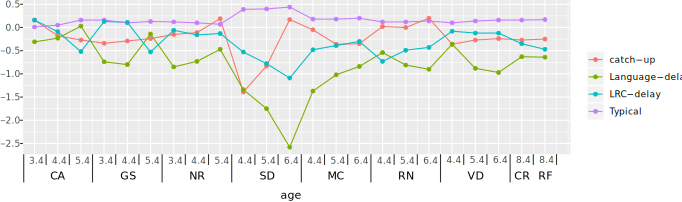
\includegraphics{Lin(2011)}
	\caption{Lin(2011)通过}
	\labfig{Lin(2011)}
\end{figure*}
	
上面的这个实验提到了一种叫混合增长模型的统计技术,我们简要介绍一下它.\reffig{Boscardin(2008)}是Boscardin(2008)的一项研究的结果,这个实验的数据分析就是用的这个模型.最大的图中,可以看到这个数学模型很好地把孩子分成两个亚类型,类型内的孩子比较接近,但是类型间的孩子相差较远;而且这些孩子中,有些孩子斜率相同,起点不同;有些孩子起点相同,斜率不同;也有可能起点不一样斜率也不一样.这就是用到复杂的统计,得到了非常丰富的信息.所以对于数学和统计学习一定要下尽全力,我们不仅要有最精细的实验设计,也要有最复杂的统计分析手段,这样才能做最好的研究,只是大多研究者醒悟的比较晚,若你现在还有心去学数学,那就立马去学吧!

\begin{figure*}
	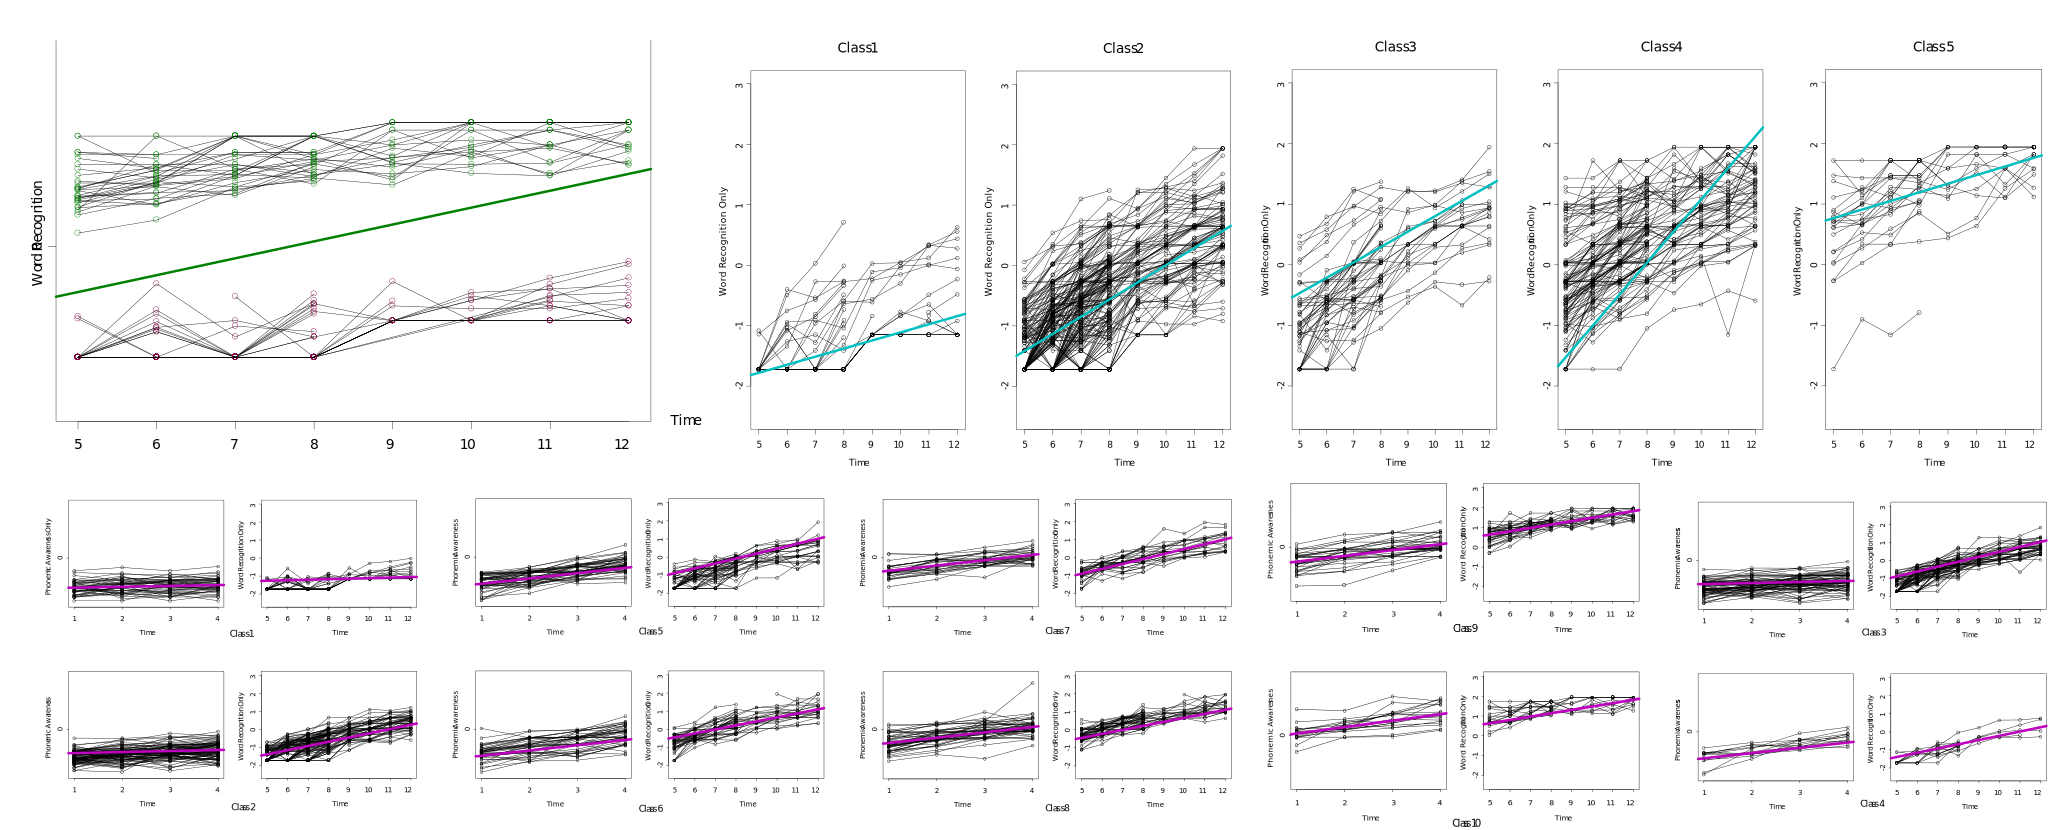
\includegraphics{Boscardin(2008)}
	\caption{Boscardin(2008)}
	\labfig{Boscardin(2008)}
\end{figure*}


前面介绍的部分实验用到了比较新的技术,一方面在工具上,针对于脑研究,像ERP/FMRI/眼动仪都是非常好的研究工具,它们帮助我们从更深层次探讨人脑的奥秘;另一方面,新的统计技术也让研究可以更精确的得出结果,包括已经写入大多课本的多重回归、路径分析、结构方程,也有上面提到的混合增长模型.不论这些手段多么的眼花缭乱,一定要注意,实质仍然是实验设计.比如下面这个实验,虽然仍然是行为学实验,不过实验设计非常有趣,非常漂亮地得到了结论.

\begin{marginfigure}
	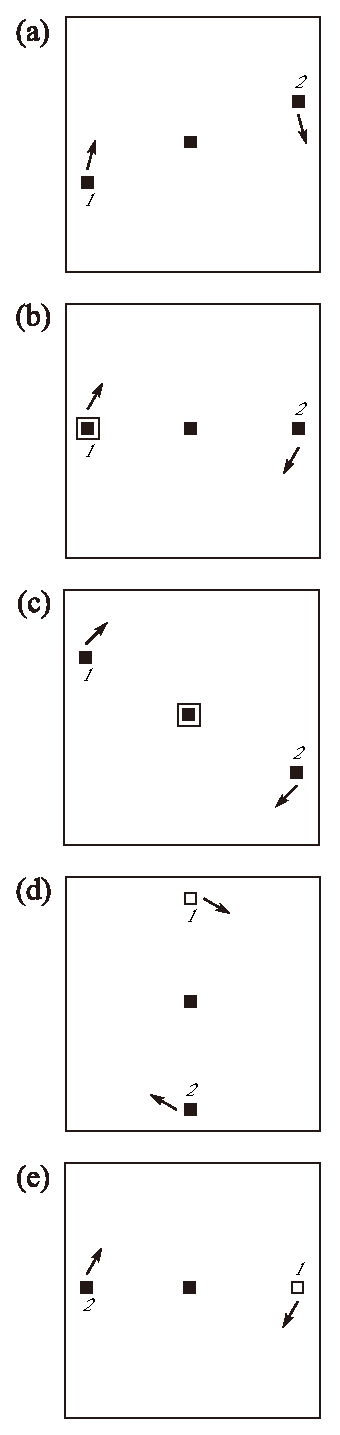
\includegraphics{Tipper(1991)}
	\caption{Tipper(1991)发现了基于物体的注意在返回抑制中相比基于空间的注意更具优势}
	\labfig{Tipper(1991)}
\end{marginfigure}

Tipper(1991)研究了注意中的返回抑制现象(inhibitation of return),所谓返回抑制,大体上是说对于我们注意过空间的某个区域,再次对其注意需要付出更多努力,在行为上的表现就是需要花费更多时间去重新注意.这点在学生看书时表现的很常见,在看完一本书后,我们好像有一种不知道哪里来的抗拒心理让我们不愿意复习.

Tipper想知道的是,我们到底是不愿意再注意注意过的物体,还是不愿意注意注意过的空间位置?若二者都存在抑制效应,哪种注意更占优势呢?\reffig{Tipper(1991)}是他的研究.初始状态a,有三个方块在视野中,方块1、方块2和中间的方块.1和2顺时针旋转到水平时(b),1闪烁,继续旋转到c后中间方块闪烁,然后等到旋转到e,此时1和2的位置和b中正好相反,然后1再次闪烁或者2闪烁,记录这次闪烁到按键间的反应时,发现被试更加难以注意1,说明了基于物体的注意在返回抑制中更有优势.

心理学研究的发展:
实验心理学:拥有严密的实验控制
教育与社会心理学:大样本+统计

复杂实验设计和多元统计的结合

推论统计——从样本推断到总体,不用
1有限的现象:可以观察到全体样本
2可以直接观察:DNA螺旋

统计假说:一种推论形式,可基于不完整的信息检验科学假说的真伪

方差分析的基本思想
对一组数据的描述:集中、离散
X1: 7 5 4 10 4
X2: 10 1 1 15 3
mean:6 6
range:4-10 1-15
var: 26 156

$$
	t=\frac{X_1-X_2}{S_P}
$$

变异是否存在?

施加处理:一致性变化(组内变化没变,组间有变)

随机分配被试来保证实验前被试同质

$$
	F=\frac{MS_effect}{MS_error}
$$

下面应该是一个随机误差,所有处理效应要和误差效应相比,



\section{实验中变异的控制}
所谓变异(variance),就是对数据离散情况的衡量.和方差(variance)是一个词,不过实验中的变异含有三种变异

\textbf{1.使系统变异最大}
	\begin{itemize}
		\item 选取适当的自变量水平,使自变量水平的改变所引起的变异能在因变量中反映出来
		\item 选择对自变量的变化敏感的因变量
	\end{itemize}

这个实验中,一个是10,000条,一个是20,000条
因变量:容易形成正态分布
愿意买哪本?1010的数据,变化不敏感,变异小
%-----------------------------------------------------------------
\textbf{2.控制无关变异}
所有可能做自变量的因素均可能成为因素均可能成为无关变异的来源,无关变量是心理学、教育学、社会学研究中最棘手的问题之一.

上面大:例如研究两种教学条件对成绩的影响,实验选择两个班,但是可能两个班的学生能力不同,使得处理效应变异虚大
下面大:主要是被试带来的个体差异

这个实验中随机分配
指导语的描述一模一样,由不同文字引起的带走了

有五种控制无法变异的基本方法:

\begin{itemize}
	\item 随机化:随机分配被试
	\item 消除:i不是一个好方法,比如性别会影响,就只研究男性
	\item 匹配:基本上都是一样的
	\item 附加自变量
	\item 统计控制
\end{itemize}
%-----------------------------------------------------------------
\textbf{3.使误差变异最小}
误差指的是在实验中没有控制的变异:
主要来自于两个:处理单元内被试间的个体差异,我们知道这个是行为学实验中最主要的差异,
测量误差
尽量在实验设计中控制,实在控制不了的用统计控制 

实验设计的评价:内部效度(稳定性、控制无法变异)、外部效度

\section{假设检验的基本思想}
F分布的基本假设
\begin{itemize}
	\item 因变量观测值大体服从正态分布,如果数据不可能符合正态分布,就不能用F检验
	\item 变异的同质性:由随机分配保证,是一个最基本的假设,因为我们根本就不做前测,只做后测
	加实验处理只是变了组间变异,实验后的组间变异也反应了处理前的组内变异
	\item 独立性:每一个观测值独立于其它观测值 
\end{itemize}

实验设计模型及其假设:变异的构成
一次观测就只有一个观察值,但是怎么知道这个观察值有哪些组成的?这个模型就是指导这件事,
如:
$$
Y_{ij}=\mu +\alpha_j + \varepsilon_{i(j)}
$$

$$
SS_{total}=SS_{within\_group}+SS_{between\_group}
$$


误差是一个平均数为0的随机变量,不是一个定向的变化


实验设计的基本过程:
1提出问题和假说的形成
问题特征:探索两个或多个变量间的关系
问题的可检验性:研究该问题的方法和手段已经解决或初步解决
Science 290 ,1582-1585(2000) 有意思的问题,在以前是没法做的,婴儿没法报告
问题所包含的变量是可以检验并可以操作化的(操作定义)
怎么操作世界知识违反操作化?非常精巧化

\section{实验中变量的实别}
变量的选择能否回答想解决的问题?
符合:1研究的理论假说/实验设计和统计的要求

\textbf{被试固有特性}:被试在实验前就有的,不太可能改变和操纵,通常分类
严格地来说,追踪的研究能得到严格的因果关系吗?
最严格的因果关系是操纵和改变自变量,引起心理或行为上的变化
有些情况下没有办法做这个
但是又没有办法做,已经是最好的了
通常在实验中还会加一个可以操控的,不会让自变量只有被试固有特性,

\textbf{被试的暂时特性}:心理学严重最丰富,最具特色的自变量.操纵外部刺激引起心理变化,不是完全外部,引起的心理变化正好是想研究的问题,但是比较难以操纵,需要找到非常好的操作定义.

可操作、可改变的
不可操作、不可改变的

自变量的数量:与问题、统计方法有关
水平的数量:动机的那个例子

主要意义次要次要意义,定SOA,43
主要意义一直维持激活,次要意义有一个上升下降的曲线


因变量:可以看到的
必须随着自变量的变化而变化
可以转化为数据

1)对自变量的变化最敏感:字典中
2)实验中选取的观测量应该可靠,得出稳定的结果
3)大体上正态分布,人的行为、生理大体上都符合正态分布,但是如果数据就不可能服从正态分布就不要用方差分析
4)可行性上考虑

Keenan(2001)自我面孔实别

无关变量

操作定义:变量必须用测量或操作它们的步骤来定义
用事物可观察、可测量的特征把研究变量具体化,它清楚地讲明与栽些现象独特联系的可观测的准则

意义:
1、对研究结果评价:同意研究结果必须先接受操作定义
2、有利于研究间交流:在前人基础上重复或修改实验
3、保障可重复性

获得方式:
1、使用现有信息:性别、教育程度、智力
2、操作创建一种形态:让被试进入实验后让其脑子发生变化,最重要
3、通过前测、评定、记录获得信息,如语义相关

Rosler(2001)

Loftus(1974)看相同的视频, 只是问题的词不同
The possible speed when the two cars

心理学研究中的道德问题——诚信
2005年有一个韩国科学家 黄禹锡 胚胎干细胞提取 编造数据 Science 撤销文章

实验无法重复的原因:
1)报告不真实:
1990然后,美国艾奥瓦大学医学部内科一名高级研究员进行了一系列实验来验证某种物质对毛细血管扩张的影响.在最后报告数据的时候,他仅保留了那些支持其假说的数据,而排除了与假说不相吻后的数据.

美化学家撤销7篇论文
碳-氢活化实验结果无法重复,美国纽约哥伦比亚大学化学教授Dalibor Sames宣布撤销在《美国化学学会期刊》《有机快报》等杂志上的7篇论文. Sames教授曾被认为是碳-氢活化领域的先锋,他的研究小组大大推进了该领域的发展.撤销论文的原因是,实验室的其他研究人员无法重复文中的结果.

2)实验控制
无关变量掺在F的上面还是下面都不好

方法的描述要细致到别人可以重复的地步








